\documentclass[11pt,a4paper,twoside,openright]{bookest}
% \usepackage[margin=1.2in,nomarginpar]{geometry}

\setlength{\textwidth}{455pt}
% \setlength{\oddsidemargin}{22pt}
% \setlength{\evensidemargin}{22pt}
% \setlength{\marginparwidth}{35pt}
% \setlength{\voffset}{0pt}
% \setlength{\hoffset}{0pt}

% \typeout{tw: \the\textwidth}
% \typeout{os: \the\oddsidemargin}
% \typeout{es: \the\evensidemargin}
% \typeout{mw: \the\marginparwidth}


\usepackage[table]{xcolor}
\usepackage[utf8]{inputenc}
%brackets 
\usepackage{amssymb}
\usepackage{polski}
\usepackage[polish]{babel}
\usepackage{graphicx}
\usepackage{pdfpages}
\usepackage{fancyhdr}
\usepackage{import}
\usepackage{wrapfig}

\author{Patryk Lisik}

\definecolor{tab1}{gray}{0.94}
\definecolor{tab2}{rgb}{1, 1, 1}

%bigger frac
\newcommand\ddfrac[2]{\frac{\displaystyle #1}{\displaystyle #2}}


\setlength{\headheight}{15pt}


\begin{document}
    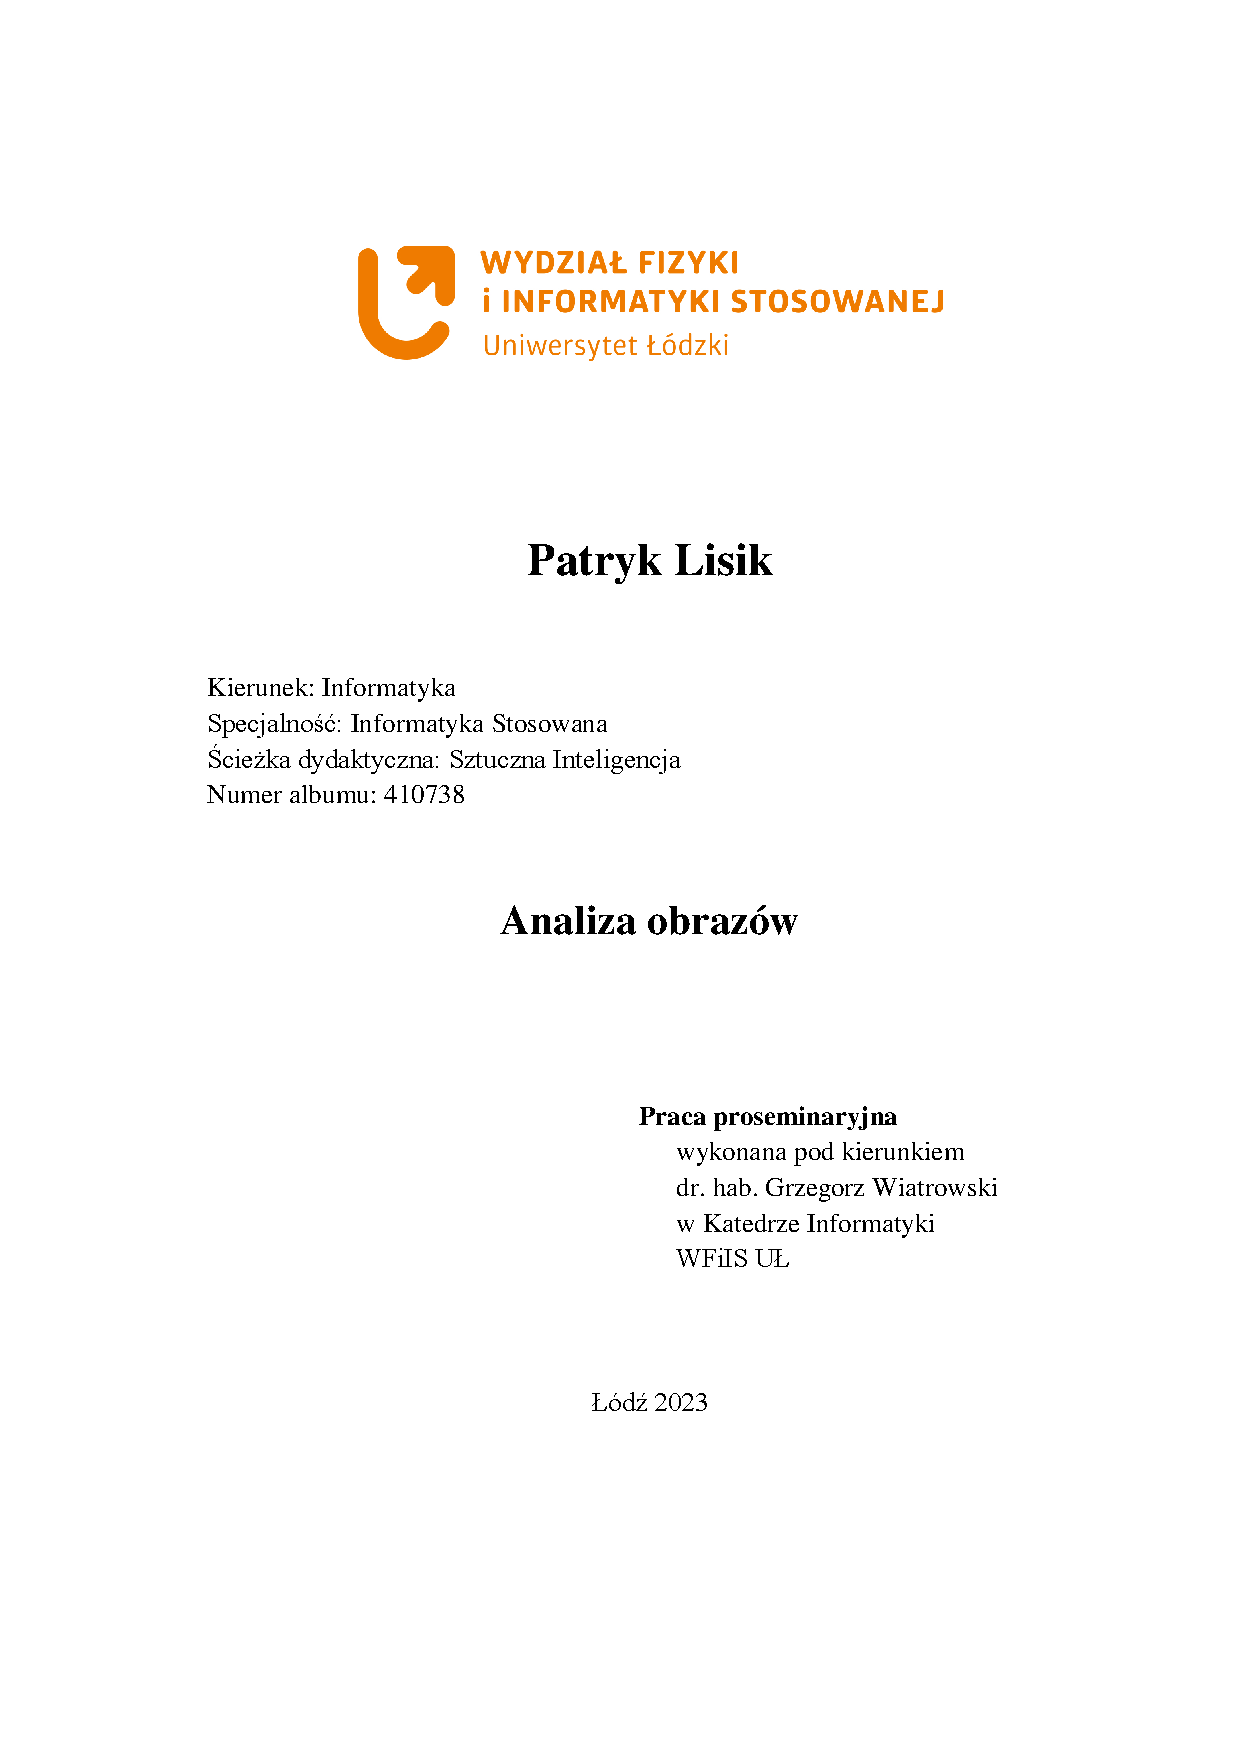
\includepdf[pages={1}]{AnalizaObrazowStronaTytulowa.pdf}
    \delimitershortfall=-1pt

    \tableofcontents



    \chapter{Wstęp}\label{ch:wstep}
    W ostatnich latach sztuczna inteligencja i jej zastosowanie do przetwarzania obrazów zyskały na ogromnej popularności.
Jednym z wyzwań, jakie towarzyszą temu postępowi, jest problem detekcji obrazów zmodyfikowanych przez sztuczną inteligencję.
W dzisiejszych czasach, gdy coraz więcej osób wykorzystuje narzędzia do obróbki grafiki wykorzystujące metody inteligentne, łatwo jest zmienić oryginalne zdjęcie w sposób, który wygląda naturalny i trudny do wykrycia przez ludzkie oko.
Jednak, dzięki sztucznej inteligencji, możliwe jest wprowadzenie znacznie bardziej skomplikowanych i subtelnych modyfikacji, które są praktycznie niemożliwe do wykrycia przez człowieka.


Współczesna cyfrowa era zwiększyła zapotrzebowanie na wykrywanie obrazów zmodyfikowanych przez sztuczną inteligencję.
Wykrycie takich modyfikacji jest niezwykle ważne w wielu dziedzinach, takich jak obróbka obrazów medycznych, zabezpieczenia danych, bezpieczeństwo sieci, a także w badaniach naukowych.
Praca magisterska ta ma na celu przyczynienie się do rozwijania tej dziedziny wiedzy, poprzez wskazanie skutecznych metod detekcji i dostarczenie narzędzi umożliwiających wykrywanie obrazów zmodyfikowanych przez sztuczną inteligencję.


\section{Cel pracy}
Celem niniejszej pracy magisterskiej jest zbadanie i ocena skuteczności różnych metod detekcji obrazów zmodyfikowanych przez sztuczną inteligencję.
W ramach pracy zostaną przedstawione różne techniki i algorytmy służące do wykrywania modyfikacji obrazów, a także zostanie omówiona ich skuteczność w wykrywaniu modyfikacji wprowadzonych przez różne rodzaje sztucznej inteligencji.
Praca składać się będzie z teoretycznej części, gdzie omówione zostaną różne aspekty detekcji modyfikacji obrazów, oraz części praktycznej, gdzie zostaną przeprowadzone eksperymenty mające na celu porównanie skuteczności różnych metod detekcji.


\section{Aktualność wyboru tematu}
Wybór tematu dotyczącego detekcji obrazów zmodyfikowanych przez sztuczną inteligencję jest bardzo aktualny z kilku powodów.

Po pierwsze, sztuczna inteligencja i jej zastosowanie do przetwarzania obrazów rozwijają się bardzo szybko, a z tego wynikają różne wyzwania, w tym wyzwanie detekcji modyfikacji obrazów.
Zastosowanie sztucznej inteligencji w obróbce obrazów pozwala na wprowadzanie coraz bardziej skomplikowanych i subtelnych modyfikacji, które mogą być praktycznie niemożliwe do wykrycia przez człowieka.
Dlatego też jest coraz bardziej istotne, aby rozwijać metody i algorytmy pozwalające na wykrywanie takich modyfikacji.
Automatyczna detekcja obrazów wygenerowanych przez AI zaczyna pojawiać na największych portalach społecznościowych jak Twitter(przykład takiego powiadomienia pokazano na~\ref{img:twitter-notification})

\begin{wrapfigure}{r}{0.5\textwidth}
    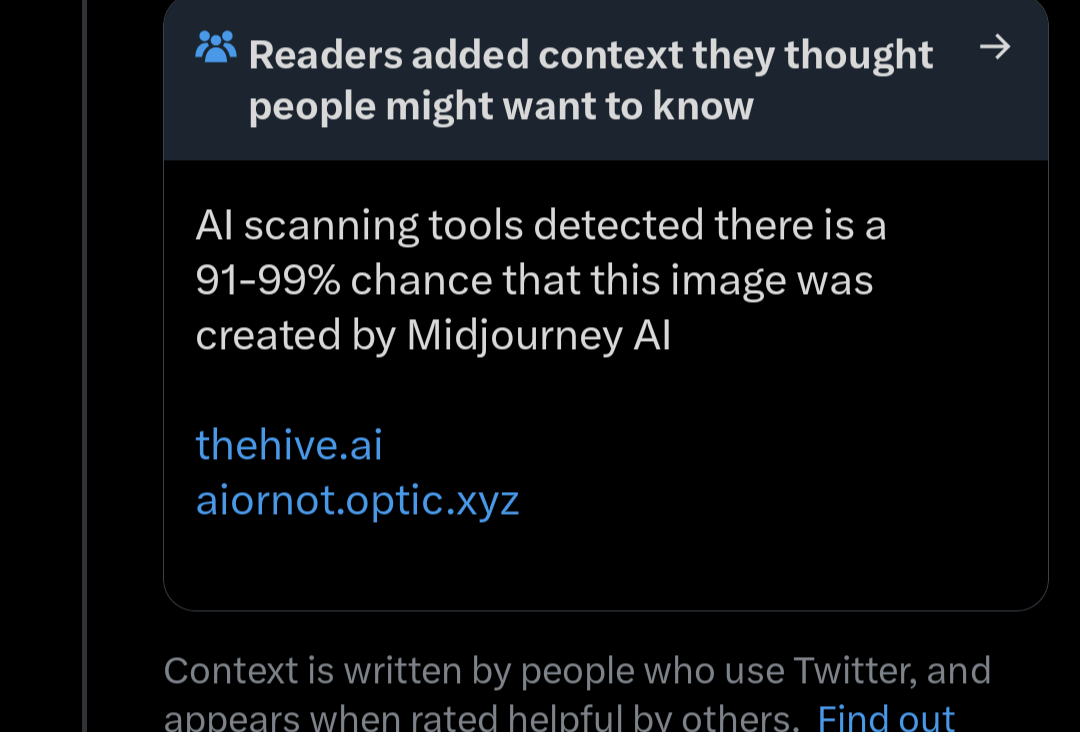
\includegraphics[width=\linewidth]{img/twitter}
    \centering
    \caption{ Powiadominie na portalu Twitter informujące o wykryciu obrazu wygenerowanego przez AI}
    \label{img:twitter-notification}
\end{wrapfigure}

Po drugie, zwiększone wykorzystanie narzędzi do obróbki obrazów, takich jak Photoshopm DeepFake cz Face2Face, sprawia, że łatwo jest zmienić oryginalne zdjęcie lub film w sposób, który wygląda naturalny i trudny do wykrycia przez ludzkie oko.
Tym samym, istnieje coraz większe zapotrzebowanie na narzędzia umożliwiające wykrywanie modyfikacji obrazów, aby zapobiegać oszustwom, np.
w kontekście fałszywych dokumentów, czy nieprawdziwych informacji w internecie.

\begin{wrapfigure}{l}{0.5\textwidth}
    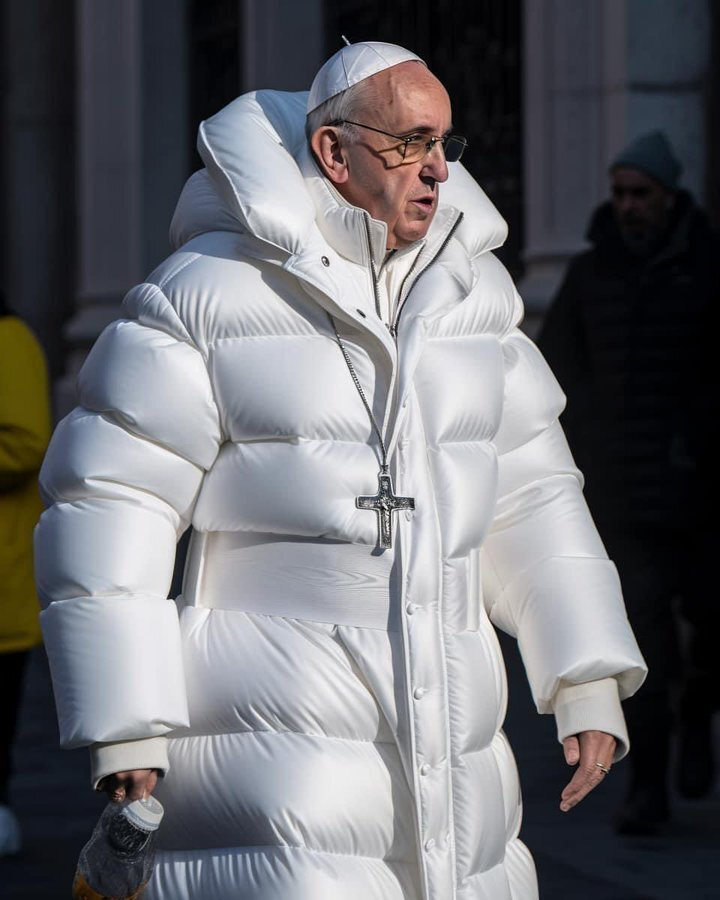
\includegraphics[width=\linewidth]{img/pope_balenciaga}
    \centering
    \caption{Wygenerowany obraz obraz znany jako "Balenciaga Pope".
    Przedstawiający papieża Franciszka noszącego kurtę wyglądającą na produkt dorgiej marki modowej Balenciaga.}
    \label{img:pope-balenciaga}
\end{wrapfigure}

Przykładem takiej kontrowersje jest obraz przedstawiający papieża Franciszka w drogiej puchowej kurtce (rysunek.~\ref{img:pope-balenciaga}).
Papież Franciszek, który jest głową Kościoła katolickiego, nie jest znany z ostentacyjnego stylu życia ani noszenia drogich ubrań.
W związku z tym, informacje sugerujące, że papież był widziany w drogiej kurtce puchowej Balenciaga, wywołały pewien skandal.
Szybko zauważono artefakty występujące na obrazie i co za tym idzie fakt że został wygenerowany przez AI. Artefakty tym na obrazie zostały omówione w rozdziale~\ref{sec:section-artifacts}.
Ten mini-skandal był jedną z przyczyn szybkiego wprowadzenia przez Twittera wspomnianych wcześniej komunikatów o obrazach wygenerowanych przez AI, pokazanych na rysunku~\ref{img:twitter-notification}.


Wreszcie, detekcja modyfikacji obrazów jest istotna w wielu dziedzinach, takich jak obróbka obrazów medycznych, zabezpieczenia danych, bezpieczeństwo sieci czy badania naukowe.
W związku z tym, rozwój metod i algorytmów umożliwiających wykrywanie modyfikacji jest bardzo istotny dla postępu w tych dziedzinach.


Podsumowując, wybór tematu dotyczącego detekcji obrazów zmodyfikowanych przez sztuczną inteligencję jest bardzo aktualny, ponieważ rozwój sztucznej inteligencji i narzędzi do obróbki obrazów, wraz z rosnącym zapotrzebowaniem na wykrywanie modyfikacji, sprawiają, że rozwijanie metod i algorytmów w tym zakresie jest niezwykle ważne.

    \chapter{Przegląd istniejących rozwiązań generowania obrazu}\label{ch:przeglad-istniejacych-rozwiazan-generowania-obrazu}
    \usepackage{wrapfig}

\section{Rozwiązania 'text to image'}
    Metody przekształcania tekstu na obraz, znane również jako `text-to-image', są obszarem badań związanych z generowaniem obrazów na podstawie opisów tekstowych~\cite{creativity_of_text_to_image}. Ta dziedzina łączy w sobie technologie z zakresu uczenia maszynowego, przetwarzania języka naturalnego i sztucznej inteligencji w celu tworzenia realistycznych wizualizacji na podstawie tekstu opisującego sceny, przedmioty lub koncepty.

    Głównym celem metod text-to-image jest zrozumienie semantyki zawartej w opisie tekstowym i przekształcenie go w obraz, który jest zgodny z opisem.
    Metody te mają szerokie zastosowanie w dziedzinach takich jak grafika komputerowa, projektowanie gier, reklama, tworzenie treści wizualnych i wiele innych.

    W ostatnich latach zanotowano znaczny postęp w dziedzinie text-to-image, dzięki rozwojowi zaawansowanych modeli generatywnych, takich jak CLIP i sieci generatywne przeciwstawne (GAN). Te modele uczą się na ogromnych zbiorach danych obrazów i tekstów, a następnie są w stanie generować realistyczne obrazy na podstawie nowych opisów tekstowych.

    Metody text-to-image mają wiele praktycznych zastosowań.
    Mogą być wykorzystywane do generowania ilustracji do książek, tworzenia grafik reklamowych, tworzenia wirtualnych światów w grach komputerowych czy wspomagania procesów projektowania i tworzenia wizualizacji. Mają również potencjał do tworzenia barwnych i wciągających treści wizualnych na podstawie prostych opisów tekstowych.

    Niemniej jednak generowanie obrazów na podstawie tekstu jest wciąż wyzwaniem, zwłaszcza jeśli chodzi o zachowanie spójności i realizm generowanych obrazów. Istnieją różne podejścia i techniki, takie jak wykorzystanie architektur sieci neuronowych, uwzględnienie kontekstu semantycznego, zastosowanie mechanizmów uwagi czy wykorzystanie danych treningowych do uczenia modeli. Badacze nadal pracują nad doskonaleniem tych metod, aby osiągnąć lepsze wyniki i generować jeszcze bardziej realistyczne obrazy na podstawie opisów tekstowych.

    \subsection{CLIP (ang.  \textit{Contrastive Language–Image Pre-training})}
    CLIP (Contrastive Language–Image Pre-training) to technologia opracowana przez OpenAI i przedstawiona w pracy badawczej opublikowanej w styczniu 2021 roku~\cite{CLIP}.
    Jej podejście polega na wykorzystaniu języka naturalnego w celu poprawy ogólności i odporności modeli uczenia głębokiego do zadań klasyfikacji obrazów. Badacze są w stanie osiągnąć wyniki na najwyższym poziomie w wielu testach, korzystając z ustawienia zero-shot, co jest niezwykle imponujące.

    Główna idea stojąca za CLIP polega na wspólnym wstępnym uczeniu modelu języka neuronowego i modelu klasyfikacji obrazów za pomocą ogromnej ilości danych obrazowych pobranych z Internetu wraz z odpowiednimi podpisami.

% Na poniższym obrazie „Koder tekstu” reprezentuje model języka, a „Koder obrazu” model klasyfikacji obrazów.
% Obrazek pochodzi z oryginalnego blogu OpenAI.


    Celem uczenia jest skonstruowanie macierzy, w której każda wartość reprezentuje miarę podobieństwa między każdą parą podpowiedzi i obrazów - obliczaną jako $I\cdot T$ na obrazku - i wykorzystanie jej do uczenia modelu językowego i wizualnego, tak aby maksymalizować wartości w pozycjach odpowiadających poprawnym param. Na przykład, jeśli tekst na pozycji 0 brzmi „pepper the aussie pup”, a obraz na pozycji 0 reprezentuje konkretną treść, CLIP nauczy oba modele tworzyć reprezentacje, które maksymalizują ich podobieństwo.

    Po zakończeniu tego procesu wstępnego szkolenia można użyć wstępnie nauczonych modeli wizualnych do wygenerowania reprezentacji dla dowolnego obrazu wejściowego i porównać je z kilkoma osadzeniami tekstowymi uzyskanymi z różnych podpowiedzi za pomocą modelu językowego.
    Wybierana jest reprezentacja tekstowa o maksymalnej wartości podobieństwa, która najlepiej reprezentuje treść na obrazie.
    Dzięki tej technice można użyć tysiąca klas ImageNet jako zdań i rozwiązać zadanie klasyfikacji w ustawieniu zero-shot.
    Zero-shot to test rozpoznawania klas, których nie ma bezpośrednio w zbiorze treningowym, a wiedza o nich jest pozyskiwana pośrednio przez naukę przypadków które znajdują się w zbiorze treningowym.
    CLIP opiera się na dużej liczbie prac dotyczących transferu zero-shot i uczeniu z nadzorem językA naturalnego.
    Pomysł na uczenie bez danych sięga ponad dekadę, ale do niedawna był głównie badany w zakresie widzenia komputerowego jako sposób na uogólnianie na niewidoczne kategorie obiektów.
    Kluczowym spostrzeżeniem było wykorzystanie języka naturalnego jako elastycznego przestrzeni predykcyjnej umożliwiającej uogólnianie i transfer.

    CLIP może być stosowany do niemal dowolnych zadań klasyfikacji wizualnej.
    Na przykład, jeśli zadaniem zbioru danych jest klasyfikacja zdjęć psów i kotów, sprawdzamy dla każdego obrazu, czy model CLIP przewiduje, że tekstowa opis „zdjęcie psa” lub „zdjęcie kota” jest bardziej prawdopodobnie z nim skojarzony.

    CLIP wstępnie szkoli koder obrazu i koder tekstu w celu przewidzenia, które obrazy zostały skojarzone z którymi tekstami zbiorze danych.
    Następnie wykorzystujemy to zachowanie, aby przekształcić CLIP w klasyfikator zero-shot.
    Zamieniamy wszystkie klasy zbioru danych na podpisy, takie jak „zdjęcie psa”, a następnie przewidujemy klasę podpisu, który CLIP uważa za najlepiej dopasowany do danego obrazu.

    CLIP został zaprojektowany w celu rozwiązania kilku głównych problemów w standardowym podejściu głębokiemu uczeniu w zakresie widzenia komputerowego:

    \begin{description}

        \item[Kosztowne zbiory danych] Głębokie uczenie wymaga dużej ilości danych, a modele wizyjne tradycyjnie były szkolone na ręcznie oznakowanych zbiorach danych, które są kosztowne w tworzeniu i dostarczają nadzoru tylko dla ograniczonej liczby ustalonych koncepcji wizualnych. Zestaw danych ImageNet, będący jednym z największych wysiłków w tej dziedzinie, wymagał zatrudnienia ponad 25 000 pracowników do oznakowania 14 milionów obrazów dla 22 000 kategorii obiektów. W przeciwieństwie do tego CLIP uczy się na podstawie par tekst-obraz dostępnych publicznie w Internecie. Redukcja potrzeby drogich, dużej skali oznaczonych zbiorów danych była szeroko badana w poprzednich pracach, zwłaszcza uczeniu bez nadzoru, metodach kontrastowych, podejściach samoszkolnych i modelowaniu generatywnym.

        \item[Wąskie zakresy] Modele oparte o uczenie głębokie jak ImageNet są skuteczne w przewidywaniu stosunkowo małej ilości kategorii(około 1000).
        Jeśli chcemy wykonać jakiekolwiek inne zadanie, osoba zajmująca się uczeniem maszynowym musi zbudować nowy zestaw danych, dodać warstwę wyjściową i dostrajać model.
        W przeciwieństwie do tego CLIP może być dostosowany do wykonywania różnorodnych zadań klasyfikacji wizualnej bez konieczności dodatkowego szkolenia.
        Aby zastosować CLIP do nowego zadania, wystarczy zamienić klasy zbioru danych na podpisy tekstowe i wybrać najbardziej prawdopodobny podpis dla danego obrazu.
        CLIP jest elastycznym klasyfikatorem zero-shot, który potrafi generalizować do nieznanych klas bez ponownego szkolenia.

        \item[Przenoszenie wiedzy między domenami] CLIP został wstępnie szkolony na różnorodnych zestawach danych obrazowych i tekstowych, co umożliwia przenoszenie wiedzy między różnymi domenami.
        Na przykład, jeśli model jest wstępnie szkolony na dużej ilości obrazów architektonicznych i tekstów opisujących architekturę, można go przenieść na nowe zadania związane z architekturą, takie jak klasyfikacja stylów architektonicznych lub rozpoznawanie budynków.

    \end{description}~\subsection{Stabilna dyfuzja)}

    Stabilna dyfuzja (ang. \textit{Stable diffusion} w kontekście generowania obrazów odnosi się do zastosowania procesów dyfuzji stabilnych do generowania nowych obrazów o wysokiej jakości i różnorodności~\cite{ramesh2022hierarchical, seneviratne2022dalle}.
    Metoda ta wykorzystuje własności dyfuzji stabilnej do stopniowego wprowadzania losowych zmian w początkowym obrazie, prowadząc do ewolucji i generowania nowych wariantów.

    Proces generowania obrazów przy użyciu Stable Diffusion zwykle rozpoczyna się od początkowego obrazu, który może być losowo wygenerowany lub wybrany spośród istniejących obrazów treningowych.
    Następnie, poprzez kolejne kroki dyfuzji, wprowadzane są losowe zmiany w pikselach obrazu.

    Kluczowym aspektem Stable Diffusion jest wykorzystanie ogólnych rozkładów stabilnych, które mają właściwość `ciągłości skalowej'.
    Oznacza to, że zmiany wprowadzane w pikselach mają charakter skalowalny, co pozwala na kontrolowane generowanie różnorodnych obrazów.
    Proces dyfuzji stabilnej umożliwia stopniowe wprowadzanie tych zmian, prowadząc do wytworzenia nowych tekstur, kształtów i struktur obrazów.

    Przy generowaniu obrazów za pomocą Stable Diffusion istotne jest również wprowadzenie mechanizmu sterowania procesem.
    Może to obejmować kontrolowanie tempo dyfuzji, aby określać tempo zmian i ewolucję obrazu.
    Może również obejmować sterowanie parametrami rozkładów stabilnych, takich jak indeks stabilności czy skala, co pozwala na dostosowanie charakterystyk generowanych obrazów.

    Metoda Stable Diffusion w generowaniu obrazów oferuje wiele możliwości, zarówno w zakresie tworzenia realistycznych tekstur i detali, jak i eksplorowania kreatywnych wariantów.
    Wykorzystanie dyfuzji stabilnej pozwala na generowanie wysokiej jakości obrazów, które są zarazem zróżnicowane i nieprzewidywalne.
    To podejście znajduje zastosowanie w dziedzinach takich jak generowanie grafiki komputerowej, sztuka generatywna, czy projektowanie graficzne.

\section{Rozwiązania oparte o generatywne sieci współzawodniczące -- GAN}


GAN (Generative Adversarial Network) to rodzaj architektury sieci neuronowych, który składa się z dwóch głównych komponentów: generatora i dyskryminatora.
GAN-y są wykorzystywane do generowania nowych danych, takich jak obrazy, dźwięki czy tekst, które są podobne do danych treningowych.

Generator w GAN-ie jest odpowiedzialny za generowanie nowych próbek danych na podstawie losowych wejść, zwanych wektorami szumowymi.
    Początkowo generator generuje losowe próbki, które nie są podobne do danych treningowych.
    Wraz z postępem uczenia, generator stara się tworzyć coraz bardziej realistyczne próbki, które przypominają rzeczywiste dane treningowe.

Dyskryminator w GANie ma za zadanie rozróżnianie między rzeczywistymi danymi treningowymi a próbkami generowanymi przez generator.
Jest to sieć neuronowa binarnego klasyfikatora, który stara się określić, czy dana próbka pochodzi z danych treningowych czy została wygenerowana przez generator.
Dyskryminator jest trenowany w procesie uczenia maszynowego w celu poprawnego klasyfikowania próbek.

Podstawową ideą GAN-a jest trening zarówno generatora, jak i dyskryminatora w równoległych procesach, które konkurują ze sobą.
Generator stara się generować jak najbardziej realistyczne próbki, aby oszukać dyskryminatora, podczas gdy dyskryminator stara się coraz lepiej rozróżniać prawdziwe dane od próbek wygenerowanych przez generator.
Proces ten jest iteracyjny i odbywa się poprzez optymalizację wag sieci neuronowych generatora i dyskryminatora w celu osiągnięcia równowagi między nimi.

Jednym z największych osiągnięć GAN-ów jest możliwość generowania wysokiej jakości i realistycznych danych, które trudno odróżnić od rzeczywistych.
GANy znalazły szerokie zastosowanie w dziedzinach takich jak generowanie obrazów, syntezowanie dźwięków, generowanie tekstów czy tworzenie grafiki komputerowej.
Stanowią one również podstawę dla zaawansowanych technologii takich jak DeepFake.

W kontekście generowania obrazów na podstawie tekstu wcześniej wspomniany CLIP znalazł swoje pierwsze znaczące zastosowanie w systemach generowania obrazów opartych na GAN~\cite{creativity_of_text_to_image}.
CLIP był używany jako składnik dyskryminatora w GAN\@.
CLIP może kierować komponentem generatora w celu stworzenia cyfrowych obrazów najlepiej odpowiadających danemu tekstowemu poleceniu.
Wkrótce po wydaniu przez OpenAI CLIP w styczniu 2021 roku, entuzjaści sztucznej inteligencji stworzyli systemy oparte na GAN+CLIP, które miały na celu generowanie sztuki cyfrowej.\     Ryan Murdoch stworzył `Big Sleep', kombinację GAN o nazwie BigGAN i CLIP. To zainspirowało Katherine Crowson do połączenia jeszcze potężniejszej sieci neuronowej (VQGAN) z CLIP. Kombinacja VQGAN i CLIP była bardzo popularna w 2021 roku i stała się jedną z standardowych technik generowania dzieł sztuki, dopóki nie została zastąpiona przez systemy oparte na stabilnej dyfuzji.
Można argumentować, że VQGAN–CLIP odegrał kluczową rolę w rozwoju powstającej dziedziny sztuki tekstowo-obrazowej.


\section{Zamiana twarzy}
Postępy w cyfryzacji ludzkich twarzy stały się podstawą nowoczesnych narzędzi do edycji obrazów twarzy. Narzędzia edycji można podzielić na dwie główne kategorie: modyfikację tożsamości i modyfikację wyrazu twarzy. Oprócz ręcznej edycji twarzy przy użyciu narzędzi takich jak Photoshop, w ostatnich latach zaproponowano wiele automatycznych podejść. Najbardziej znaczącą i powszechnie stosowaną techniką modyfikacji tożsamości jest zamiana twarzy, która zyskała znaczną popularność, ponieważ lekkie systemy są teraz zdolne do działania na telefonach komórkowych. Dodatkowo, dostępne są teraz techniki rekonstrukcji twarzy, które zmieniają wyraz twarzy osoby poprzez przeniesienie wyrazu źródłowej osoby na cel. Ninejsza praca przedswai dwa zautomatyzowane podjeścia deeepFake i Face2Face.

\subsection{DeepFake}
DeepFake to technologia, która wykorzystuje sztuczną inteligencję do tworzenia manipulacji wideo, w których twarze i głosy ludzi są zamieniane lub manipulowane w sposób realistyczny~\cite{DeepFakegithub}.
Przykad takiej podmiany pokazano na rysunku~\ref{img:deepfake-example}.
Termin `DeepFake' jest połączeniem słów `deep learning' (głębokie uczenie maszynowe) i `fake' (fałszywy), co odzwierciedla zastosowanie zaawansowanych algorytmów uczenia maszynowego w celu tworzenia realistycznych fałszerstw.

\begin{wrapfigure}{r}{0.5\textwidth}
    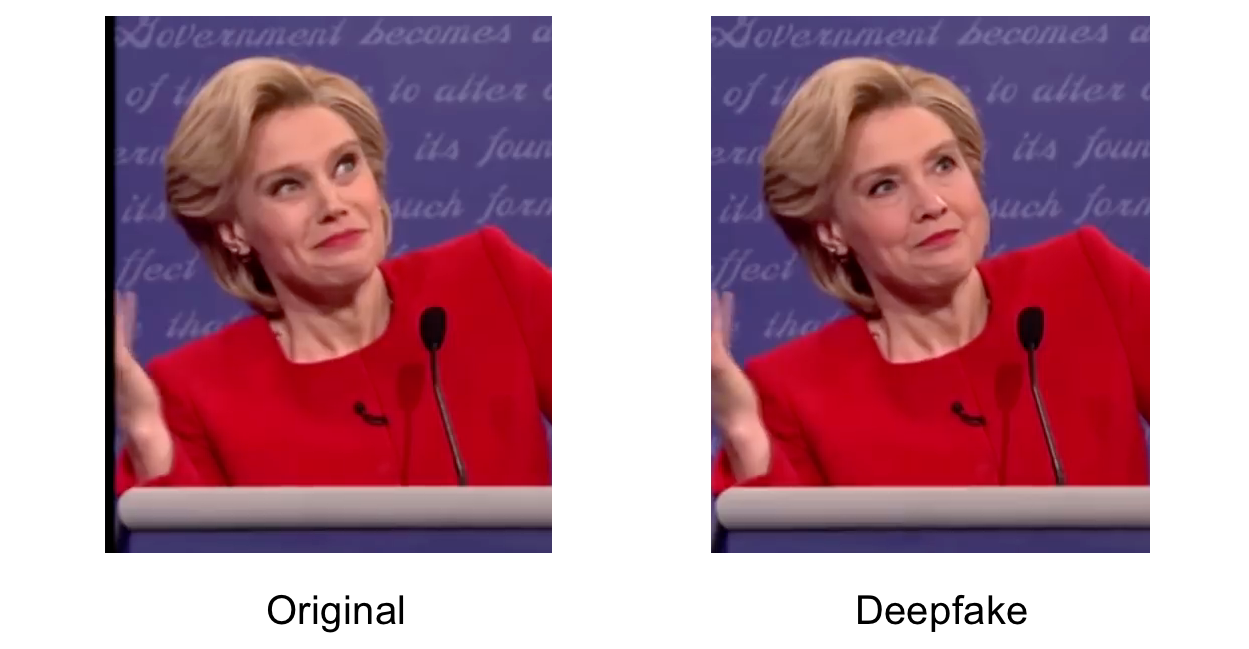
\includegraphics[width=\linewidth]{img/deepfake_example}
    \centering
    \caption{ Przykład zamiany twarzy za pomocą Deepfake. Zauważalny jest znaczny spadek ekspresyjności twarzy. Źródło:~\cite{mesoNet} }
    \label{img:deepfake-example}
\end{wrapfigure}

Głównym elementem technologii DeepFake jest sieć neuronowa, znana jako generatywna sieć przeciwnika (GAN)\cite{tolosana2020deepfakes}.
Proces tworzenia DeepFake zazwyczaj obejmuje dwa kluczowe etapy: trening i generację. W etapie treningowym sieć neuronowa jest uczona na dużej ilości danych, które zawierają pary obrazów i/lub nagrań dźwiękowych, reprezentujących oryginalne twarze i głosy osób, które mają zostać podmienione.
Na podstawie tych danych sieć neuronowa uczy się modelować charakterystyki twarzy i głosów.

Po etapie treningu następuje etap generacji, w którym sieć neuronowa jest używana do stworzenia nowego wideo, w którym twarze lub głosy są manipulowane.
Na podstawie podanych danych wejściowych (np. obrazów twarzy lub nagrania dźwiękowego), sieć generuje wideo, w którym twarze zostają podmienione na twarze osób z danych wejściowych lub głosy zostają podmienione na głosy innych osób. W rezultacie powstaje wideo, które wygląda i/lub słucha się tak, jakby osoba na wideo naprawdę mówiła lub miała określoną twarz.

DeepFake ma zarówno pozytywne, jak i negatywne aspekty. Z jednej strony może być wykorzystywany w dziedzinach takich jak przemysł filmowy, reklamowy czy rozrywkowy, aby tworzyć realistyczne efekty specjalne i efekty wizualne. Z drugiej strony, DeepFake może stanowić poważne zagrożenie, gdy jest wykorzystywany do oszustw, szantażu, fałszywych informacji, czy manipulacji politycznych.
Może wpływać na wiarygodność w mediach i stanowić wyzwanie dla autentyczności informacji.

Ze względu na swoje rosnące znaczenie i potencjalne zagrożenia, badania nad wykrywaniem DeepFake i opracowywanie metod rozpoznawania i ograniczania tego rodzaju manipulacji stają się coraz bardziej istotne dla bezpieczeństwa i zaufania wobec mediów i technologii cyfrowych.

\subsection{Face2Face}

Face2Face to system rekonstrukcji twarzy, który przenosi wyrażenia z wideo źródłowego na wideo docelowe, jednocześnie zachowując tożsamość osoby docelowej~\cite{thies2020face2face}.

\begin{figure}[h]
    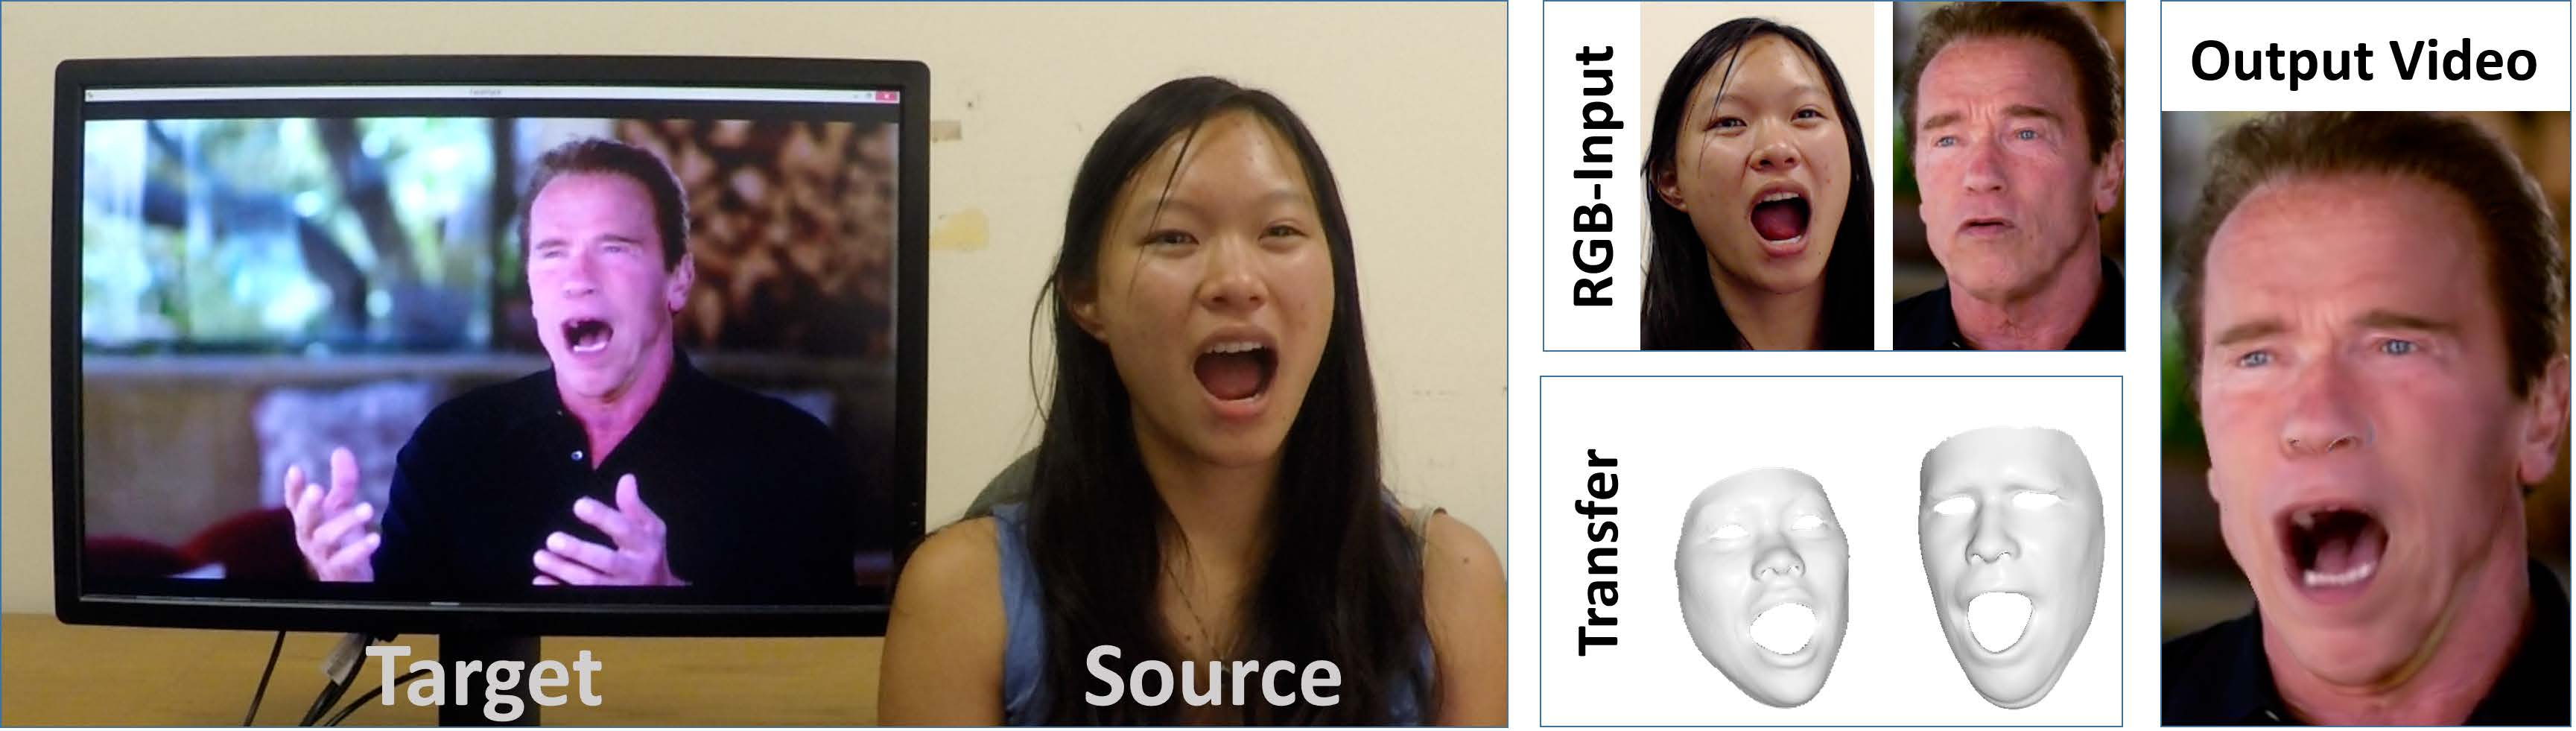
\includegraphics[width=0.9\linewidth]{img/Face2Face}
    \caption{ Działanie Face2Face Źródło:~\cite{thies2020face2face}}
    \label{img:face2face}
\end{figure}

Oryginalna implementacja Face2Face opiera się na dwóch strumieniach wideo, które są ręcznie wybierane jako kluczowe klatki.
Rysunek~\ref{img:face2face} pokazuje działanie omawianej technologi.
Twarz Arnolda Schwarzeneggera została zmieniona na bazie twarzy innej osoby.
Te klatki są wykorzystywane do generowania gęstej rekonstrukcji twarzy, która może być następnie użyta do odtworzenia twarzy przy różnym oświetleniu i wyrażeniach.
W pracy, dostosowujemy podejście Face2Face w celu automatycznego tworzenia manipulacji rekonstrukcyjnych.
Każde wideo jest przetwarzane w fazie wstępnej. Wykorzystujemy pierwsze klatki, aby uzyskać tymczasową tożsamość twarzy (czyli model 3D) i śledzimy wyrażenia na pozostałych klatkach. W celu wyboru kluczowych klatek wymaganych przez podejście, automatycznie wybieramy klatki z najbardziej skrajnym kątem twarzy. Na podstawie tej rekonstrukcji tożsamości śledzimy całe wideo, obliczając dla każdej klatki parametry wyrażenia, sztywnego położenia i oświetlenia, tak jak w oryginalnej implementacji Face2Face. Generujemy wynikowe wideo rekonstrukcji, przenosząc parametry wyrażeń źródłowych każdej klatki (czyli 76 współczynników Blendshape) na wideo docelowe. Szczegółowe informacje na temat procesu rekonstrukcji można znaleźć w oryginalnym artykule~\cite{thies2020face2face}.

Face2Face jest potężnym narzędziem, które umożliwia przenoszenie wyrażeń twarzy z jednego wideo na drugie, przy zachowaniu tożsamości osoby docelowej. Jego automatyczna wersja, zaimplementowana w ramach pracy, pozwala na masowe przetwarzanie wideo i tworzenie manipulacji rekonstrukcyjnych w sposób efektywny i skalowalny.

Badacze stosują nową, gęstą, bezmarkerową metodę przechwytywania wyrazu twarzy opartą na jednookularowych danych RGB, podobnie jak w najnowocześniejszych metodach. Jednak głównym wkładem jest odzwierciedlanie twarzy w czasie rzeczywistym, zamiast przekazywania wyrazu twarzy do wirtualnych postaci CG. W przeciwieństwie do poprzednich podejść do odzwierciedlania, które działają w trybie offline, celem jest przekazywanie wyrazu twarzy źródłowej osoby przechwyconej przez czujnik RGB do docelowej osoby w czasie rzeczywistym.
Docelowa sekwencja może być dowolnym wideo jednookularowym, na przykład wcześniejszym materiałem pobranym z serwisu YouTube z wyrazem twarzy. Celem jest modyfikacja docelowego wideo w fotorealistyczny sposób, tak aby manipulacje były praktycznie niemożliwe do zauważenia.
Wiernie fotorealistyczne odzwierciedlanie wyrazu twarzy stanowi podstawę wielu zastosowań, na przykład wideo-konferencji, gdzie strumień wideo może być dostosowany do ruchów twarzy tłumacza lub twarze mogą być przekonująco dubbingowane na język obcy.

W metodzie najpierw odtwarzana jest identyczność kształtu docelowej osoby za pomocą nowej globalnej, nieliniowej metody opartej na modelu, wykorzystując wcześniej nagrane sekwencje treningowe.
Ponieważ ten etap wstępny jest wykonywany globalnie na zestawie klatek treningowych, można rozwiązać niejednoznaczności geometryczne, które są typowe dla rekonstrukcji jednookularowej.
W czasie rzeczywistym śledzone są wyrazy twarzy zarówno osoby źródłowej, jak i docelowej przy użyciu metody analizy i syntezy opartej na statystycznym modelu wyrazu twarzy. Udowodniono, że dokładność śledzenia przy użyciu danych RGB jest porównywalna z najnowocześniejszymi metodami, nawet z metodami śledzenia online opartymi na danych głębi.
W celu przekazywania wyrazów twarzy od osoby źródłowej do docelowej w czasie rzeczywistym proponuje się nowe funkcje transferu, które skutecznie stosują transfer deformacji bezpośrednio w przestrzeni wyrazu twarzy o niskiej wymiarowości. Do ostatecznej syntezy obrazu odtwarzana jest twarz docelowej z przekazanymi współczynnikami wyrazu twarzy i komponowana jest z tłem wideo docelowej osoby z uwzględnieniem oszacowanego oświetlenia środowiska. Wprowadzana jest również nowa metoda syntezowania wnętrza ust oparta na obrazach, która generuje realistyczne wewnętrzne usta przez pobieranie i deformowanie najlepiej dopasowanych kształtów ust z wcześniej przygotowanej sekwencji próbkowania.
Ważne jest zauważenie, że zachowuje się wygląd kształtu ust docelowej osoby, podczas gdy istniejące metody albo kopiują obszar ust osoby źródłowej na docelową, albo renderują ogólny model zębów, co prowadzi do niejednoznacznych rezultatów.

\section{Artefakty generowanych obrazów}
\label{sec:section-artifacts}

Obrazy generowane przez modele oparte na Stable Diffusion i GAN-ach mogą czasami wykazywać pewne artefakty, które wynikają z charakterystyki tych metod.
Oto kilka powszechnych artefaktów, które można zaobserwować w tego rodzaju obrazach:

\begin{wrapfigure}{r}{0.4\textwidth}
    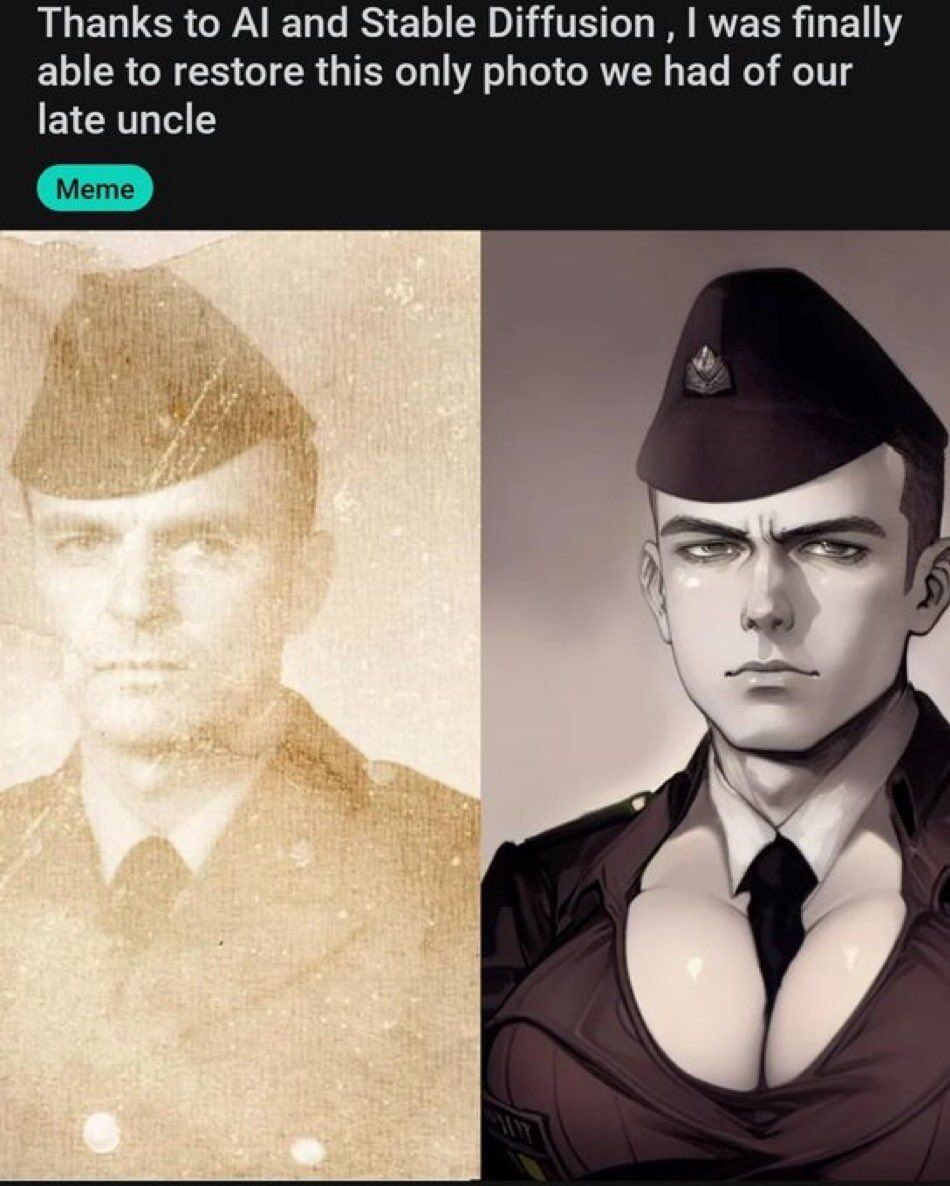
\includegraphics[width=\linewidth]{img/falied-image-restoration}
    \centering
    \caption{ Błędna regeneracja obrazu przez Stable Diffusion. Jest to przykład tzw. halucynowania}
    \label{img:falied-restoration}
\end{wrapfigure}


\begin{description}

    \item[Szumy lub zniekształcenia] Obrazy generowane przez modele mogą wykazywać różne rodzaje szumów lub zniekształceń, takich jak piksele o nietypowych kolorach, nieostry obraz lub nieprawidłowe tekstury.
    Te artefakty mogą być wynikiem niedoskonałości modelu i trudności w perfekcyjnym odwzorowaniu złożonych wzorców obrazów rzeczywistych.

    \item[Nieprawidłowe proporcje] Czasami modele mogą generować obrazy o nieprawidłowych proporcjach, na przykład deformacje twarzy lub nietypowe kształty obiektów.
    Może to wynikać z ograniczeń modelu w odwzorowaniu precyzyjnych proporcji i proporcji obiektów.

    \item[Artefakty tekstury] Generowanie realistycznej i spójnej tekstury może być wyzwaniem dla modeli opartych na Stable Diffusion i GAN-ach.
    Mogą występować nieprawidłowe tekstury lub nieciągłości w generowanych obrazach, co prowadzi do artefaktów teksturalnych, takich jak niewłaściwe wzory, rozmazane krawędzie lub nieprawidłowe detale.

    \item[Nadmierne dopasowanie danych treningowych] Modele GAN, szczególnie w przypadku niedostatecznej różnorodności w zbiorze treningowym, mogą czasami nadmiernie dopasować się do danych treningowych.
    Może to prowadzić do powtarzających się wzorców lub `klonowania' obiektów, gdzie generowane obrazy wyglądają podobnie lub są zbyt podobne do obrazów treningowych.

    \item[Niewłaściwe kontekstowe informacje] Modele są oparte na danych treningowych, które mogą mieć ograniczenia w zakresie reprezentacji różnorodnych kontekstów.
    W rezultacie generowane obrazy mogą zawierać niewłaściwe kontekstowe informacje, co prowadzi do nieprawidłowych lub niedopasowanych elementów w obrazach.
    Popularna nazwa tego zawiaska to halucynowanie.
    Tego typu sytuację pokazano na obrazie~[\ref{img:falied-restoration}]

\end{description}

\begin{wrapfigure}{l}{0.4\textwidth}
    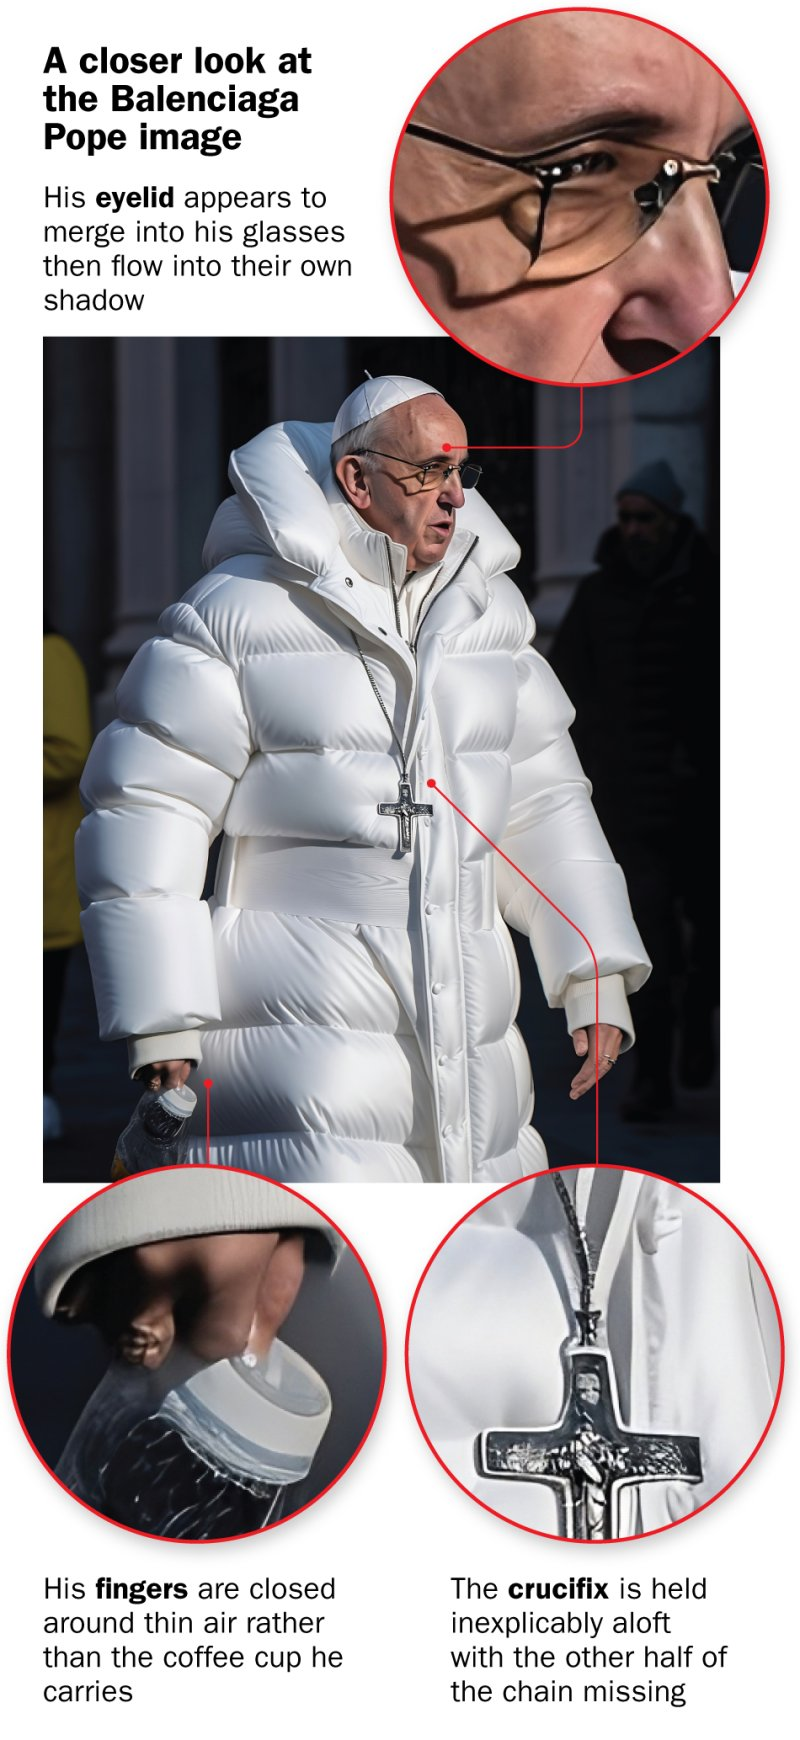
\includegraphics[width=\linewidth]{img/Pope-annotation}
    \centering
    \caption{ Typowe artefakty które można odnaleźć na obrazach generowanych przez metody sztucznej inteligencji. Źródło:~\cite{howToSpotBalenciagaPope} }
    \label{img:pope_annotation}
\end{wrapfigure}

Gdy przyjrzeć się uważnie obrazowi `Balenciaga Pope'(rysunek~\ref{img:pope-balenciaga}, można dostrzec kilka wyraźnych oznak jego powstania za pomocą sztucznej inteligencji.
Krzyż wiszący na jego piersi jest niepokojąco uniesiony, zaledwie biała puchowa kurtka zamiast drugiej połowy łańcucha.
W jego prawej ręce znajduje się coś, co wydaje się zamazanym kubkiem z kawą, ale palce, zamiast trzymać kubek, zamykają się wokół powietrza.
Powieka niezrozumiale łączy się z okularami, które z kolei przechodzą w swój własny cień.
Przybliżenia na te artefakty obrazu pokazano na rysunku~\ref{img:pope_annotation}.


Aby rozpoznać obraz generowany przez sztuczną inteligencję, często warto przyjrzeć się tym skomplikowanym detalom.
Jak palce, włosy czy w tym przypadku krzyż.
Krzyż nie powinien unosić się w powietrzu bez łańcucha go podtrzymującego.
Okulary i cień za nimi nie są jednym obiektem.
Obecność tego typu artefaktów pozwala wykrywać obrazy wygenerowane przez sztuczną inteligencję.

    \chapter{Istniejące rozwiązania wykrywania obrazów niewytworzonych przez człowieka}\label{ch:istniejace-rozwiazania-wykrywania-obrazow-niewytworzonych-przez-czowieka}
    \section{Detekcja przetworzonych twarzy -- FaceForensics++}
Artykuł `FaceForensics++' rozpatruje szereg istotnych zagadnień w dziedzinie detekcji manipulacji twarzy~\cite{rossler2019faceforensics++}.
Przede wszystkim, przedstawia zautomatyzowany benchmark do wykrywania manipulacji twarzy w przypadku losowej kompresji, co umożliwia standaryzowane porównanie różnych metod detekcji.
Benchmark ten obejmuje także bazową ocenę przeprowadzaną przez ludzi, co umożliwia porównanie skuteczności automatycznych systemów detekcji do wyników uzyskanych przez ekspertów.

\begin{figure}[h]
    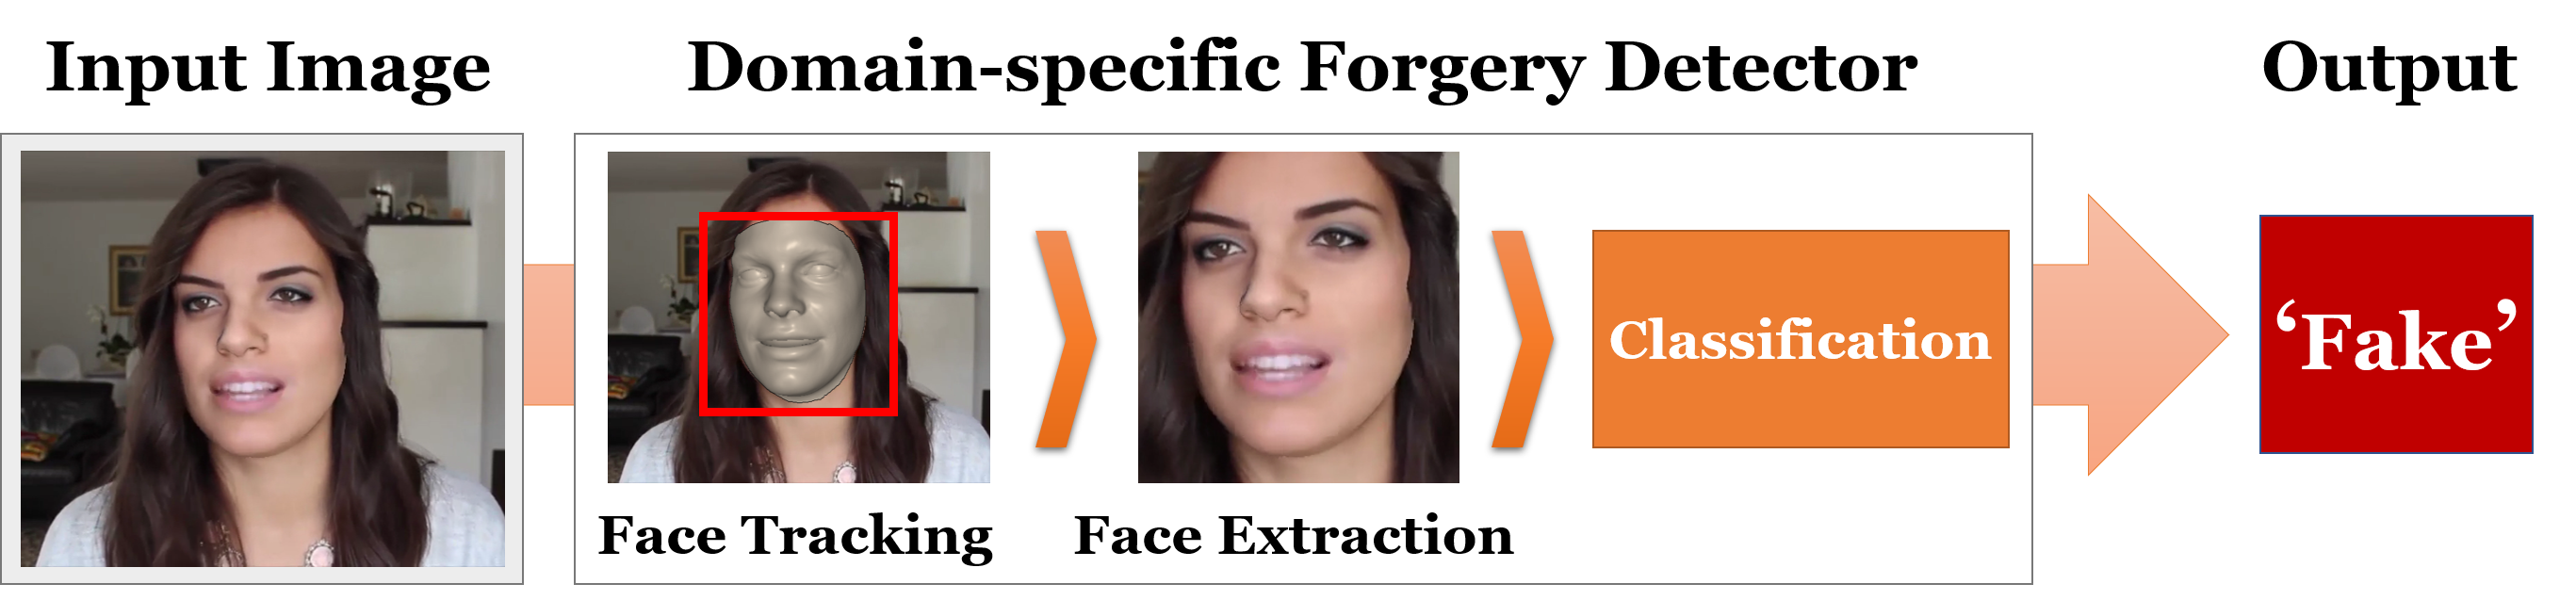
\includegraphics[width=0.9\linewidth]{img/FF++detection_pipeline}
    \caption{ Wizualne przedastwanie kroków działania FaceForensics++.
    Obraz wejściowy jest przetwarzany przez metodę śledzenia twarzy; informacje są wykorzystywane do wyodrębnienia obszaru obrazu pokrytego twarzą. Następnie ten obszar jest podawany na wejście nauczonej sieci klasyfikacyjnej, która generuje predykcję.
    Źródło~\cite{rossler2019faceforensics++}:}
    \label{img:FFPileline}
\end{figure}

Kolejnym ważnym wkładem naszego artykułu jest stworzenie innowacyjnego i obszernego zbioru danych do nauki.
Zbiór ten zawiera ponad 1,8 miliona obrazów pochodzących z 1000 filmów, które przedstawiają manipulowane obrazy twarzy.
Co więcej, dla każdego manipulowanego obrazu posiadamy również oryginalne obrazy stanowiące dane referencyjne.
Dzięki temu zbiór ten umożliwia nadzorowane uczenie się systemów detekcji, co pozwala na poprawę ich skuteczności.

Nasz artykuł obejmuje również obszerną ocenę najnowocześniejszych detektorów fałszerstw, zarówno opartych na metodach manualnych, jak i na uczeniu maszynowym.
Przeprowadziliśmy tę ocenę w różnych scenariuszach, co pozwoliło nam zrozumieć i porównać skuteczność tych detektorów w różnych kontekstach.
Dzięki temu dostarczamy wglądu w najlepsze obecnie dostępne metody detekcji manipulacji twarzy.

Ostatecznie, artykuł przedstawia najnowocześniejszą metodę detekcji fałszerstw, stworzoną specjalnie do manipulacji twarzy.
Ta metoda wykorzystuje najnowsze osiągnięcia w dziedzinie detekcji manipulacji obrazów, aby zapewnić wysoką skuteczność w wykrywaniu manipulacji twarzy.

Wszystkie te wkłady mają na celu rozwinięcie dziedziny detekcji manipulacji twarzy i dostarczenie narzędzi oraz wiedzy, które przyczynią się do poprawy bezpieczeństwa w obszarze rozpoznawania twarzy i zwalczania manipulacji obrazów.

W obecnych metodach manipulacji obrazem twarzy, które są uważane za najlepsze w swojej kategorii, demonstrujemy, że można je wykryć za pomocą szkoleniowych detektorów fałszerstw.
Szczególnie zachęcające jest to, że trudny przypadek niskiej jakości wideo może być rozwiązany za pomocą podejścia opartego na uczeniu maszynowym, gdzie ludzie i ręcznie opracowane cechy napotykają trudności.

Autorzy FaceForresic++ stworzyli standaryzowany benchmark dla dalszych prac.
Wszystkie dane obrazowe, szkoleniowe modele oraz benchmark są publicznie dostępne i są już wykorzystywane przez innych badaczy.
W szczególności `zero-shot learning' ma duże znaczenie, gdyż w miarę pojawiania się nowych metod manipulacji, konieczne jest opracowanie metod umożliwiających wykrywanie fałszerstw przy niewielkim lub żadnym dostępnym zbiorze danych treningowych.


\section{Lokalizowanie anormalnych cech obrazów -- ManTra-Net}

\begin{figure}[h]
    \centering
    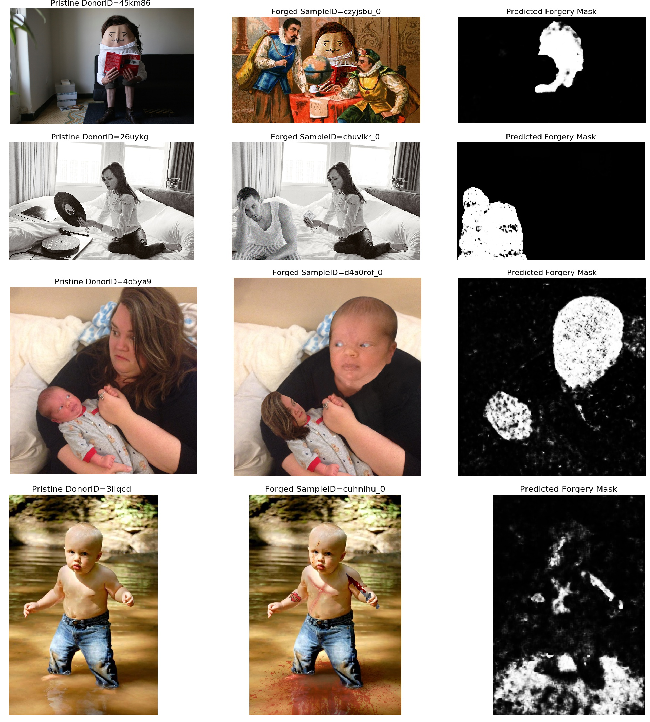
\includegraphics[width=0.7\linewidth]{img/mantra-net-example}
    \caption{Obraz iluctrujacy działanie MantraNet. Pierwsza kolumna od lewj pokazuje niezmieniony obraz.
    Kolejna kolumna pokazuje zmieniony obraz będoący wejsćiem do sieci. Piewsza kolumna od prawej to wyjście z sieci.
    Wyjściem z sieci jest obraz w odcieniach szarosci, gdzie kolor czarny oznacza brak zmiany a kolor biały oznacza że zmiana jest pewna.
    Źródło~\cite{ManTraNet}:}
    \label{fig:mantra-net}
\end{figure}

ManTra-Net to sieć neuronowa, która wykonuje zarówno detekcję, jak i lokalizację manipulacji bez dodatkowego przetwarzania wstępnego i poprzedzającego~\cite{ManTraNet}.
Jest to sieć w pełni konwolucyjna, która obsługuje obrazy o dowolnych rozmiarach oraz wiele znanych rodzajów fałszerstw, takich jak przycinanie, kopiowanie, usuwanie, poprawianie, a nawet nieznane typy manipulacji.
Działanie modelu pokazano na obrazie~\ref{fig:mantra-net}.

Artykuł ma trzy istotne wkłady.
Po pierwsze, pokazuje zbieżną metodę uczenia bez nadzoru, które pozwala na naukę wykrywania śladów manipulacji obrazem poprzez klasyfikację 385 rodzajów manipulacji obrazem.
Po drugie, formułujemy problem lokalizacji fałszerstw jako problem lokalnego wykrywania anomalii, wykorzystując cechę Z-score, która pozwala na wykrywanie lokalnych anomalii, oraz proponują nowatorskie rozwiązanie z wykorzystaniem długotrwałej pamięci krótkoterminowej(LSTM) w celu oceny lokalnych anomalii.
Na koniec przeprowadzono eksperymenty różnicowe, aby systematycznie optymalizować projekt sieci.
Wyniki eksperymentalne dowodzą ogólnego zastosowania, odporności i przewagi ManTra-Net, nie tylko w pojedynczych typach manipulacji/fałszerstw, ale także w ich skomplikowanych kombinacjach.

ManTra-Net to potężne narzędzie, które umożliwia wykrywanie i lokalizację różnych rodzajów manipulacji obrazów.
Zdolność do obsługi obrazów o różnych rozmiarach i różnych typów manipulacji czyni go wszechstronnym i przydatnym w różnych scenariuszach.
Wyniki eksperymentalne potwierdzają skuteczność i niezawodność tej technologii, co stanowi istotny wkład w dziedzinie analizy manipulacji obrazów.


\section{Detekcja przetworzonych twarzy –- MeasoNet}

MeasoNet to model do automatycznego i efektywnego wykrywania manipulacji twarzy w wideo, ze szczególnym uwzględnieniem dwóch niedawno stosowanych technik generowania sfałszowanych wideo: Deepfake i Face2Face~\cite{mesoNet}.
Tradycyjne techniki kryminalistyki obrazu zazwyczaj nie są odpowiednie dla wideo ze względu na kompresję, która silnie degraduje dane.
Dlatego w niniejszej publikacji stosuje się podejście oparte o dwie sieci o niewielkiej liczbie warstw, aby skupić się na właściwościach obrazów.
Ocena tych szybkich sieci przeprowadzana jest zarówno na istniejącym zbiorze danych, jak i na zbiorze danych stworzonym z wideo dostępnych online.
Twórcy wykorzystali test stworzony przez zespół FaceForenzic++.
Testy wykazują bardzo wysoką skuteczność wykrywania, wynoszącą ponad 98\% dla Deepfake i 95\% dla Face2Face.


W tej sekcji przedstawiane są kilka skutecznych podejść do radzenia sobie zarówno z problemem Deepfake, jak i Face2Face.
Okazało się, że te dwa problemy mogą być skutecznie rozwiązane przy użyciu pojedynczej sieci.
Jednak dzięki podobnej naturze fałszerstw, identyczne struktury sieciowe dla obu problemów mogą dawać dobre rezultaty.

Proponuje się wykrywanie sfałszowanych wideo twarzy poprzez umieszczenie metody na mezoskopowym poziomie analizy.
Rzeczywiście, mikroskopowe analizy oparte na szumach obrazu nie mogą być zastosowane w kontekście skompresowanego wideo, gdzie szum obrazu jest znacznie zdegradowany.
Podobnie na wyższym poziomie semantycznym ludzkie oko ma trudności w rozróżnianiu sfałszowanych obrazów, zwłaszcza gdy obraz przedstawia ludzką twarz.
Dlatego proponuje się przyjęcie pośredniego podejścia, polegającego na wykorzystaniu głębokiej sieci neuronowej o niewielkiej liczbie warstw.

Dwie następujące architektury osiągnęły najlepsze wyniki klasyfikacji spośród wszystkich testów, przy niskim poziomie reprezentacji i zadziwiająco niskiej liczbie parametrów.
Opierają się one na dobrze działających sieciach do klasyfikacji obrazów [14, 23], które na przemian wykorzystują warstwy splotowe i pooling do ekstrakcji cech, oraz gęstą sieć do klasyfikacji.


\section{Analzia poziomu błędów (ang. \textit{Error level analysis})}

Error Level Analysis (ELA) to metoda analizy obrazów, która służy do wykrywania zmian i manipulacji w cyfrowych obrazach.
Polega na porównywaniu poziomów kompresji w różnych obszarach obrazu, aby zidentyfikować obszary o potencjalnych zmianach.

Proces ELA polega na kompresowaniu oryginalnego obrazu cyfrowego z użyciem określonego algorytmu kompresji, na przykład JPEG, a następnie porównaniu otrzymanego obrazu skompresowanego z oryginalnym obrazem.
Różnice między tymi dwoma wersjami obrazu wskazują obszary, które mogły ulec manipulacji lub edycji.

Opis procesu ELA:

Konwersja do formatu JPEG: Oryginalny obraz jest konwertowany na format JPEG z wybranym poziomem kompresji.
Kompresja JPEG jest stratnym algorytmem kompresji, który usuwa niektóre szczegóły obrazu i wprowadza pewne artefakty.

Porównanie poziomów kompresji: Porównuje się otrzymany skompresowany obraz z oryginalnym obrazem, piksel po pikselu.
Różnice w poziomach kompresji wskazują obszary, które mogą ulec manipulacji.

Wygenerowanie mapy błędów: Na podstawie różnic w poziomach kompresji generowana jest tzw.
mapa błędów, która wizualizuje obszary o potencjalnych zmianach.
Obszary o wysokim stopniu zmian mają jasne lub intensywne kolory, podczas gdy obszary bez zmian są bardziej jednolite.

Interpretacja wyników: Analiza mapy błędów pozwala zidentyfikować obszary, które mogły ulec manipulacji.
Na przykład, obszary o wysokim stopniu zmian mogą wskazywać na dodanie, usunięcie lub zmianę pewnych elementów w obrazie.

ELA ma swoje ograniczenia i nie jest narzędziem idealnym.
Wyniki analizy ELA mogą być podatne na pewne błędy interpretacyjne, zwłaszcza w przypadku obrazów o różnych stopniach detali, tekstur i złożoności.
Ponadto, analiza ELA może wykrywać zmiany w kompresji, ale nie jest w stanie jednoznacznie ustalić, jakie dokładnie zmiany zostały wprowadzone w obrazie.

Mimo tych ograniczeń analiza poziomu błędów jest jednym z narzędzi stosowanych w cyfrowej obróbce zdjęć i badaniu autentyczności obrazów, pomagając w identyfikacji potencjalnych manipulacji i zmian w obrazach cyfrowych.

    \chapter{Podsumowanie}\label{ch:podsumowanie}

    W niniejszej pracy proseminaryjnej skoncentrowano się na rozpoznawaniu obrazów generowanych przez sztuczną inteligencję oraz ich wpływie na różne dziedziny życia.
    Przeprowadzono dogłębną analizę technik i algorytmów wykorzystywanych do generowania obrazów, a następnie opisano metody rozpoznawania tych obrazów.

    Pierwszym etapem pracy było zapoznanie się z najważniejszymi technikami generowania obrazów przez AI, takimi jak generatywne modele współzawodniczące (GAN), głębokie sieci neuronowe czy autokodery.
    W oparciu o te techniki przeprowadzono szereg eksperymentów, które wykazały ogromne postępy w generowaniu realistycznych obrazów przez sztuczną inteligencję.
    Jednak równocześnie pojawiły się też obawy dotyczące możliwości manipulacji i wprowadzania dezinformacji za pomocą generowanych przez AI obrazów.

    Następnie przystąpiono do badania metod rozpoznawania obrazów wygenerowanych przez AI. Przeanalizowano różne podejścia, w tym ekstrakcję cech, uczenie maszynowe oraz analizę statystyczną.
    Wykazano, że rozpoznawanie obrazów generowanych przez AI stanowi niezwykle trudne wyzwanie ze względu na ich wysoką jakość i podobieństwo do rzeczywistych obrazów.
    Wskazano również na konieczność ciągłego doskonalenia technik rozpoznawania, aby nadążyć za postępującym rozwojem generatywnych modeli.

    Następnie omówiono różne dziedziny, w których obrazy generowane przez AI mają wpływ.
    Przeanalizowano ich zastosowanie w medycynie, sztuce, tworzeniu treści multimedialnych oraz reklamie.
    W każdej z tych dziedzin zidentyfikowano zarówno korzyści, jak i potencjalne zagrożenia.
    Obrazy generowane przez AI mają ogromny potencjał do poprawy jakości życia i rozwoju nauki, ale jednocześnie stanowią wyzwanie dla rzetelności informacji i prywatności.

    Wnioski z przeprowadzonych badań wskazują na to, że rozpoznawanie obrazów generowanych przez AI jest niezwykle ważnym zagadnieniem.
    Pomimo postępów w dziedzinie generowania obrazów przez AI, istnieje nadal wiele wyzwań związanych z rozpoznawaniem i weryfikacją ich autentyczności.
    Dlatego niezbędne jest rozwijanie bardziej zaawansowanych technik i narzędzi, które będą w stanie skutecznie rozpoznawać generowane przez AI obrazy.

    W związku z tym dalsze badania i prace w tej dziedzinie są niezwykle istotne.
    Konieczne jest opracowanie bardziej zaawansowanych algorytmów i metod rozpoznawania, które będą w stanie skutecznie odróżniać obrazy generowane przez AI od rzeczywistych obrazów.
    Ponadto rozwój systemów opartych na sztucznej inteligencji, które będą mogły wykrywać manipulacje i fałszerstwa w obrazach generowanych przez AI, będzie kluczowy dla zachowania rzetelności informacji oraz ochrony przed dezinformacją.

    Wraz z postępem technologii AI i generowania obrazów, z pewnością pojawią się nowe wyzwania i możliwości.
    Praca magisterska stanowi jedynie wstęp do tej fascynującej dziedziny i może stanowić punkt wyjścia do dalszych badań i eksploracji.
    Rozpoznawanie obrazów generowanych przez AI jest jednym z najważniejszych tematów w dziedzinie sztucznej inteligencji, które będzie miało ogromny wpływ na nasze społeczeństwo i codzienne życie.

    Ostatecznie, postęp w rozpoznawaniu obrazów generowanych przez AI jest kluczowy dla zbudowania zaufania do sztucznej inteligencji oraz zapewnienia bezpiecznego i odpowiedzialnego wykorzystania tych technologii.
    Tylko poprzez dalsze badania, innowacje i współpracę między naukowcami, instytucjami i społecznościami możemy osiągnąć postęp w tej dziedzinie i maksymalnie wykorzystać potencjał obrazów generowanych przez AI dla dobra ludzkości.
% \cite{LatentDiffusionModels, zhang2023adding,nguyen2023new,hamid2023improvised,uloli2022survey, birunda2022fake, liao2021imperceptible, nguyen2019use} 
% \cite{hsu2020deep,marra2018detection}

    \bibliographystyle{ieeetr}
    \bibliography{refs}

\end{document}
